\documentclass[border=5pt]{standalone}
\usepackage{tikz}
\usepackage{tikz-3dplot}
\usetikzlibrary{arrows.meta, 3d, perspective, calc}
\usepackage{amsmath}
\begin{document}
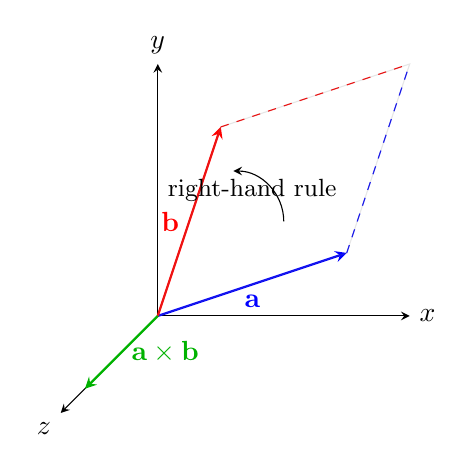
\begin{tikzpicture}[scale=0.8, >=stealth]
    % Coordinate system
    \draw[->] (0,0,0) -- (4,0,0) node[right]{$x$};
    \draw[->] (0,0,0) -- (0,4,0) node[above]{$y$};
    \draw[->] (0,0,0) -- (0,0,4) node[below left]{$z$};

    % Vectors
    \draw[->,thick,blue] (0,0,0) -- (3,1,0) node[midway,below] {$\mathbf{a}$};
    \draw[->,thick,red] (0,0,0) -- (1,3,0) node[midway,left] {$\mathbf{b}$};
    \draw[->,thick,green!70!black] (0,0,0) -- (0,0,3) node[midway,right] {$\mathbf{a} \times \mathbf{b}$};

    % Parallelogram
    \draw[blue,dashed] (3,1,0) -- (4,4,0);
    \draw[red,dashed] (1,3,0) -- (4,4,0);
    \draw[gray,opacity=0.2] (0,0,0) -- (3,1,0) -- (4,4,0) -- (1,3,0) -- cycle;

    % Right-hand rule indication
    \draw[->] (2,1.5,0) arc (0:90:0.8);
    \node at (1.5,2,0) {\small right-hand rule};
\end{tikzpicture}
\end{document}
